\documentclass[a4paper,12pt]{article}
\usepackage[osf]{mathpazo}
\usepackage{ms}
\usepackage{amsmath,amsfonts,amssymb}
\usepackage{natbib}
\usepackage{lineno}
\usepackage{graphicx}
\usepackage{caption}
\modulolinenumbers[5]
\linenumbers

\pdfminorversion=3

\makeatletter
\renewcommand{\@biblabel}[1]{\quad#1.}
\makeatother

\title{Statistical and conceptual challenges in the comparative analysis of principal components}
\author{
Josef C. Uyeda$^{1,*}$, Daniel S. Caetano$^1$, and Matthew W. Pennell$^1$
}

\date{}
\affiliation{
 $^{1}$ Department of Biological Sciences \& Institute for Bioinformatics and Evolutionary Studies, University of Idaho, Moscow, ID 83844, U.S.A.\\ 
 $^{*}$ Email for correspondence: \texttt{pseudacris@gmail.com}\\
}

\runninghead{PCA in comparative analyses}
\keywords{Phylogenetic comparative methods, principal components, Brownian motion, Ornstein-Uhlenbeck, multivariate statistics}


\begin{document}

\mstitlepage
\parindent=1.5em
\addtolength{\parskip}{.3em}
\vfill

\section{Abstract}
\begin{enumerate}
\item The macroevolutionary trajectory of any trait is almost certainly influenced by evolutionary processes acting on correlated characters. However, even when data is available for multiple traits, most current approaches for modeling trait evolution along a phylogeny only consider a single trait. Therefore, in order to apply standard comparative methods, some sort of reduction in dimensionality is necessary.

\item A common procedure for reducing the dimensionality of a multi--trait dataset is to perform Principal Components Analysis (PCA) on the traits and then analyze each PC axis as a univariate character. Two alternative approaches are widely used to obtain PC scores for species: standard PCA and ``phylogenetically corrected'' PCA. 

\item We demonstrate that failing to include phylogenetic relationships when calculating PC scores can positively mislead inferences. Specifically, even when data are simulated under Brownian motion (BM), the first several PC scores will be biased toward rapid evolution early in a clade's history, and slowed down towards the present day.

\item When performing phylogenetic PCA (pPCA), it is usually assumed that the traits have evolved under a multivariate BM model. It is unknown whether this assumption is reasonable if the actual traits have evolved under more complex scenarios. Using simulations, we find that for many common models of evolution, calculating PC scores based on a BM model is a reasonable approximation for model selection, though predictable distortions in trait distributions occur across PC scores when the generating model is not BM.

\item \emph{Synthesis:} While pPC axes may be statistically independent of one another, this should not be confused with evolutionary independence. We argue that using pPCA in macroevolutionary studies can divorce analyses from the desired evolutionary inferences. Alternative approaches for modeling multivariate data that preserve interpretability are likely to be more informative, though further statistical and conceptual innovations will be necessary for these to be more broadly applicable.
\end{enumerate} 

\newpage

\section{Introduction}
Quantitative geneticists long ago recognized the value and importance of studying evolution in a multivariate framework. Due to linkage, pleiotropy, coordinated selection and mutational covariance, the evolutionary response in any phenotypic trait can only be properly understood in the context of other traits. This fact is also of course well--recognized by comparative biologists. However, unlike in quantitative genetics, most of the statistical and conceptual tools for analyzing phylogenetic comparative data \citep[recently reviewed in][]{PennellHarmon} are designed for analyzing a single trait. Even classical approaches for testing for correlated evolution across a phylogeny \citep[e.g.,][]{Felsenstein1985, Grafen1989, HarveyPagel1991} model each trait as having evolved under a process that is independent of the state of the other \citep{HansenOrzack2005}. As a result of these limitations, it is often desirable to decompose a multivariate dataset into sets of statistically independent set of traits, such that each set can be analyzed with the univariate methods.

The most common method for reducing the dimensionality of the dataset is to perform Principal Components Analyses (PCA) prior to analyzing the data using phylogenetic comparative methods. The first PC axis is the eigenvector in the direction of greatest variance, the second PC axis, the second greatest variance, and so on. However, standard methods for calculating PC scores assume that the samples are independent of one another, which is hardly ever the case for comparative data. As a result of shared common ancestry, relatives are likely to share many traits and trait combinations. This fact is, of course, now almost universally recognized and conducting comparative analyses without considering the phylogenetic relationships of species is anathema to most evolutionary biologists.

However, the necessity of considering phylogeny in some types of data transformations \citep{Revell2008} is not similarly recognized and standard PCA continues to be regularly used in comparative biology. This is done with a variety of types of traits including geometric morphometric landmarks \citep[e.g.,][]{Dornburg2011, Hunt2013}, measurements of multiple morphological traits \citep[e.g.,][]{Harmon2010, BergmannIrshick2012, Weir2012, Pienaar2013, Price2014}, and climatic variables \citep[e.g.,][]{KozakWiens2010, Schnitzler2012}. We stress that the papers that we have cited here are simply examples selected from a substantial number of papers where standard PCA was used.

By far, the most frequently used method for correcting for the non--independence of species is to assume a phylogenetic model for the evolution of measured traits and incorporate the expected covariance in the calculation of the PC axes and scores \citep{Revell2008}. Revell's method (explained in detail below) assumes that the measured traits have evolved under a multivariate Brownian motion \citep[BM;][]{Edwards1964} model of trait evolution. In a brief simulation study, \citet{Revell2008} demonstrated that if the underlying model for the traits was indeed a multivariate BM model, performing standard PCA gave biased estimates of the eigenvalues, whereas pPCA did not.

In this paper, we first extend the argument of \citet{Revell2008} and demonstrate that not only are the eigenvalues obtained from PCA biased but that they are biased in a systematic and predictable way. Performing comparative analyses on standard PC axes can therefore positively mislead inference. This point has been made in other fields that deal with auto--correlated data, such as population genetics \citep{Novembre}, ecology \citep{Podani2002}, climatology \citep{Richman1986} and paleobiology \citep{Bookstein2012}. However, the connection between these previous results and phylogenetic comparative data has not been explicitly made and standard PCs continue to be widely used in the field. We hope that our paper helps change this practice.

Second, as stated above, \citet{Revell2008} assumed that the measured traits had evolved under a multivariate BM process. As the pPC scores are not phylogenetically independent \citep[][see below]{Revell2008, Polly2013}, one must use comparative methods to analyze them which will in turn require their own evolutionary model. The choice of model for the traits and the pPC scores are separate steps in the analysis \citep{Revell2008}. 
This has the potential to introduce an odd circularity into the analysis. It seems likely that misspecifying the model for the evolution of the traits might have downstream ramifications for model--based inferences of the evolution of the PCs. To our knowledge this effect has not been previously explored. Here we perform a brief simulation study to investigate whether assuming a BM model for the traits introduces systematic biases in the pPC scores when the generating model is different.  

Last, we consider the interpretation of evolutionary models fit to pPC axes and discuss the conceptual and statistical advantages and disadvantages of using pPCA compared to alternative approaches for studying multivariate evolution in a phylogenetic comparative framework. We argue that the statistical advantages of using pPC axes comes at a substantial conceptual cost and that alternative techniques are likely to be much more informative for addressing many evolutionary questions.

\section{Methods}
\subsection{\emph{Overview of pPCA}}
Before describing our analyses, we briefly overview the approach of \citet{Revell2008} for computing pPC scores for each species. In conventional PCA, a $m \times m$ covariance matrix $\mathbf{R}$ is computed from a matrix of trait values $\mathbf{X}$ for the $n$ species and $m$ traits
\begin{equation}\label{eq:rpca}
\mathbf{R} = (n-1)^{-1}(\mathbf{X} - \mathbf{1m}^\intercal)^\intercal (\mathbf{X} - \mathbf{1m}^\intercal)
\end{equation}
where $\mathbf{m}$ is a vector containing the means of all $m$ traits and $\mathbf{1}$ is a column vector of ones. We note that in many applications $\mathbf{X}$ may not represent the raw trait values; in geometric morphometrics, for example, size, translation and rotation will often be removed from $\mathbf{X}$ prior to computing $\mathbf{R}$ \citep{RohlfSlice, Bookstein1997}. The eigenvalues $\mathbf{D}$ and eigenvectors $\mathbf{V}$ of $\mathbf{R}$ are then obtained using singular--value decomposition $\mathbf{R}=\mathbf{V}\mathbf{D}\mathbf{V}^{-1}$ or some related technique. The scores $\mathbf{S}$, the trait values of the species along the PC axes are computed as
\begin{equation}\label{eq:Spca}
\mathbf{S}=(\mathbf{X} - \mathbf{1m}^\intercal)\mathbf{V}.
\end{equation}

Phylogenetic PCA differs from this procedure in two important ways \citep{Revell2008,Polly2013} . First the covariance matrix is inversely weighted by the expected covariance of trait values between taxa under a given model $\mathbf{\Sigma}$. Under a BM model of trait evolution, $\mathbf{\Sigma}$ is simply proportional to the matrix representation of the phylogenetic tree $\mathbf{C}$, such that $\Sigma_{i,j}$ is the shared path length between lineages $i$ and $j$. (We note that as only relative branch lengths matter, we can assume that the BM rate parameter $\sigma^2=$ 1, such that $\mathbf{\Sigma}=\mathbf{C}$.) Including the expected covariance between trait values essentially just re--orients the axes according to the phylogeny. Second, the space is centered on the ``phylogenetic means'' $\mathbf{a}$ of the traits rather than their arithmetic means, which can be computed following \citet{RevellHarmon2008}:
\begin{equation}\label{eq:phymean}
\mathbf{a}=[(\mathbf{1}^\intercal \mathbf{\Sigma}^{-1} \mathbf{1})^{-1} 
\mathbf{1}^\intercal \mathbf{\Sigma}^{-1} \mathbf{X}]^\intercal.
\end{equation}
In pPCA, Equation \ref{eq:rpca} is therefore modified as
\begin{equation}\label{eq:rppca}
\mathbf{R} = (n-1)^{-1}(\mathbf{X} - \mathbf{1a}^\intercal)^\intercal \mathbf{\Sigma}^{-1} (\mathbf{X} - \mathbf{1a}^\intercal)
\end{equation}
Similarly, $\mathbf{S}$ can be calculated for pPCA using Equation \ref{eq:Spca} but substituting the phylogenetic means for the arithmetic means
\begin{equation}\label{eq:Sppca}
\mathbf{S}=(\mathbf{X} - \mathbf{1a}^\intercal)\mathbf{V}
\end{equation}
where again, $\mathbf{V}$ is a matrix containing the eigenvectors of $\mathbf{R}$ (in this case obtained from Equation \ref{eq:rppca}).

The properties of pPCA differ from those of PCA in two important ways \citep{Revell2008, Polly2013}. First, the scores of each pPC axis are not independent of scores on other axes. Second, the eigenvectors and eigenvalues of the pPCA are phylogenetically independent but the scores themselves are not. Both these properties imply that when testing for correlated evolution among pPC scores or between pPC scores from one axis an another trait, it is necessary analyze the pPC scores in a phylogenetic framework, just as one would with any other trait \citep{Revell2008, Polly2013}. 


\subsection{\emph{Effect of PCA on model selection under multivariate Brownian motion}}
We simulated 100 replicate datasets under multivariate Brownian motion to evaluate the effect of using standard versus phylogenetic PCA to infer the mode of evolution. For each dataset, we used \texttt{TreeSim} \citep{treesim} to simulate a phylogeny of 50 terminal taxa under a pure--birth process and scaled each tree to unit height. We then simulated a 20--trait dataset under multi-variate Brownian motion. For each simulation, we generated a positive definite covariance matrix for the multivariate BM process $\mathbf{\Sigma}$, by drawing eigenvalues from an exponential distribution with a rate $\lambda = \text{1/100}$ and randomly oriented orthogonal eigenvectors. We then used this matrix to sample a covariance matrix for the tip states 
$\mathbf{X}\sim \mathcal{N}(\mathbf{0}, \mathbf{C} \otimes \mathbf{\Sigma})$.
For each of the 100 simulated datasets, we computed PC scores using both standard methods and pPCA \citep[using the \texttt{phytools} package;][]{phytools}. We used \texttt{phylolm} \citep{HoandAne2014} to fit models of trait evolution to the original data and to all PC scores obtained by both methods. Following \citet{Harmon2010}, we considered three models of trait evolution: 1) BM; 2) Ornstein--Uhlenbeck with a fixed root \citep[OU:][]{ Hansen1997}; and 3) Early Burst \citep[EB:][]{Blomberg2003, Harmon2010}. We then calculated the Akaike weights (AICw) for each model/transformation/trait combination.

To explore the effect of trait correlation on inference, we conducted an additional set of simulations where $\mathbf{\Sigma}$ was varied from the above simulations to result in more or less correlated sets of phenotypic traits. We drew eigenvalues $\mathbf{m}$ from an exponential distribution and scaled these so that the leading eigenvalue $m_{\text{1}}$ was equal to 1. We then exponentiated this vector across a sequence of exponents ranging for $\ll$1 to $\gg$1. This gave us a series of covariance matrices ranging from highly correlated ($m_{\text{1}} = \text{1}; m_{\text{2}}, \ldots, m_{\text{20}} \approx \text{0}$) to nearly independent ($\mathbf{m} \approx \textbf{1}$), respectively. We chose the series of exponents to obtain a regular sequence of $m_{\text{1}} / \sum_{i=\text{1}}^{\text{20}} m_i$ ranging from 0.05 to 1. For each set of eigenvalues, we simulated 25 datasets and estimated the slope of the relationship between the absolute size of phylogenetically independent contrasts \citep{Felsenstein1985} and the height of the node at which they were calculated \citep[i.e., the ``node height test'' of][]{FreckletonHarvey2006}. Under OU models, this relationship is expected to be positive, while under EB models this relationship is negative.

%% Insert: Simulations of matrices with different rank

\subsection{\emph{Effect of using PCA when traits are not Brownian}}
We conducted an additional set of simulations in which we varied the underlying model for each of the traits in the dataset. Because of difficulties in efficiently simulating large multivariate datasets of covarying traits under OU or EB models, we instead simulated 20 independent traits under BM, OU and EB for 50 taxa trees (as above, but setting all eigenvalues equal to one another). Of course, this is certainly not represenative of the process that have shaped real multivariate data, considering this simple case allowed us to investigate how misspecifying the model of trait evolution can impact analyses under the simplest scenario.

For the BM simulations, we set $\sigma^2=\text{1}$. For OU, we set $\sigma^2=\text{1}$ and $\alpha=\text{2}$, such that the phylogenetic half--life log(2)/$\alpha$ \citep{Hansen2008} was equal to $\sim$ 0.35 of the total tree depth. For EB, we again set $\sigma^2=\text{1}$ and set $a$, the exponential rate of deceleration, to be log(0.02). 

As above, we fit BM, OU and EB models to the original data, PC scores and pPC scores for each simulated dataset and estimated parameters and AICw. In addition to the model--fitting and comparison, for every transformation, we applied two common diagnostic tests for deviation from BM--like evolution to all trait/PC axes. First, we calculated the slope of the node height test as described in the preceding section. Second, we characterized the disparity through time \citep{Harmon2003} using the \texttt{geiger} package \citep{geiger2}. 


\subsection{\emph{Empirical examples}}
We analyzed two comparative datasets assembled from the literature, allowing us to investigate the effects of principal components analyses on realistically structured data. First, we analyzed phenotypic evolution across the family Felidae using measurements from two independent sources --- five cranial measurements from \cite{slater_2009} and body mass and skull width from \cite{sakamoto_2010} (See Table 1 in Supporting Online Information). For the analysis, we used the supertree compiled by \cite{Nyakatura_2012}. Second, we analyzed 16 size--corrected morphometric traits in \textit{Cyprinodon} and related fishes \citep{Martin2011}. In both datasets, all measurements were linear measurements on the logarithmic scale. In both cases we conducted standard and phylogenetic PCA and examined the effect of each on model--fitting, the slope of the node--height test, and the average disparity through time. All simulations and analyses were conducting using R v3.0.2 \citep{R}. Scripts to reproduce all analyses are available at \texttt{https://github.com/mwpennell/phyloPCA}.
  
%We analyzed two comparative datasets assembled from the literature to investigate the effects of different data transformations on the analyses of real comparative data. This has the advantage that we obviously do not know the ``true'' model of evolution for the traits, it is difficult to simulate data with the structure of real data. We selected two different types of traits --- morphological and climate variables --- for which PCA is commonly used. For the morphological example, we analyzed phenotypic evolution across the family Felidae (cats). Measurements are the compilation of two independent sources --- five cranium measurements from \cite{slater_2009} and body mass and skull width from \cite{sakamoto_2010} (Online Supplementary table). For the example of climatic variables, we expanded our data to include all of Carnivora. We obtained geographical distribution for Carnivora species from GBIF database (\textit{Citation}) and world-wide climate data with 2.5 arc--minutes resolution from \cite{hijmans_2005}. For both the Felidae and Canivora datasets, we used the same recently published supertree \citep{Nyakatura_2012}, pruned down to the species in the respective datasets.

%As with the simulated data, we fit BM, OU, and EB to all traits/PC axes using the original data, standard PCA and pPCA. On each trait/transformation/model combination, we also performed the node--height test and disparity through time analysis described above. 


\section{Results}
\subsection{\emph{Effect of PCA on model selection under multivariate Brownian motion}}
Standard PCA introduces a systematic bias in the favored model across principal components. In our simulations, EB models had systematically elevated support as measured by Akaike weights for the first few components, for which it generally exceeded support for the BM model (Figure \ref{corbm}). Fitting models sequentially across PC axes 1--20 revealed a regular pattern of increasing support for BM models moving from the first toward the intermediate components, followed by increasing support for OU models among later components (which generally approached an AICw of 1). This regular pattern across trait axes was not present for either the original datasets, or for phylogenetic principal components, which found strong support for the BM model regardless of which trait was analyzed. We note that the theoretical maximum AICw for the BM model in the three--model comparison is $1/(2e^{-1} + 1) \approx$ 0.576, as BM is a special case of both OU and EB and therefore the $\Delta$AICw for these models cannot be greater than 2.   

Multivariate datasets simulated with high correlations and low effective dimensionality increased support for BM across PC axes. When the leading eigenvalue explained a large proportion of the variance, the slope of the node height test converged toward 0, indicating no systematic distortion of the contrasts through time (Figure \ref{rank}). However, when the eigenvalues of the rate matrix were more even, standard PCA resulted in a negative slope in the node height test among the first few PCs, which in turn provides elevated support for EB models. This pattern is reversed among higher PC axes, which have positive slopes between node-height and absolute contrast size, which provides elevated support for OU models (Figures \ref{rank} and \ref{nhplot}). 

\subsection{\emph{Effect of using PCA when traits are not Brownian}}
If the underlying model was either OU or EB rather than BM, then phylogenetic PCA tended to increase support for the true model relative to the original trait variables for the first few component axes (Figures \ref{oufit}, \ref{aicwbm}, and \ref{aicweb}). For example, when each of the original trait variables were simulated under an OU process, support for the OU model increased for pPC1 relative to the original trait variables. Higher principal component axes inferred a regular pattern of decreasing support for the OU model, while the last few PCs have equivocal support for either a BM or OU model (Figure \ref{oufit}, top panel). Furthermore, parameter estimation was affected by phylogenetic PCA. The $\alpha$ parameter of the OU model was estimated to be stronger than the value simulated for individual traits for the first few pPC scores and lower for the higher components (Figure \ref{alpha}). 

Examining the results from the node--height tests (Figure \ref{nhplot}) and the disparity through time analyses (Figure \ref{dttplot}) help clarify the results we observed from model comparison and parameter estimation. Under OU models, traits are expected to have the highest contrasts near the tips, whereas under EB models, traits will have the highest contrasts near the root of the tree. Under multivariate BM, standard PCA tends to select linear combinations of traits that maximize the contrasts at the root of the tree, thereby maximizing the overall variance explained across the entire dataset. Thus, the first few PCs are skewed toward resembling EB models, while the last few PCs are skewed toward resembling OU models. By contrast, the effect of pPCA on the node--height relationship depends on the generating model. When traits are evolved under an OU model, the first few pPC axes show an exaggerated pattern of high variance towards the tips. Likewise, when traits are evolved under an EB model, the first few pPC axes show an exaggerated pattern of high variance towards the root of the tree. For traits generated under both OU and EB models, the higher components resemble BM--like patterns. 

\subsection{\emph{Empirical examples}}
In the Felid dataset, the seven morphometric traits were extremely highly correlated, with the first PC explaining 96.9\% and 93.7\% of the total variation in the dataset for standard PCA and phylogenetic PCA, respectively.
%% Percent of variance explained calculated in 'phylopca.Rmd' line 258 to 262.
All raw trait axes support a BM model of evolution, and the first PC of both standard and phylogenetic PCA likewise favors a BM model of evolution (both have AICw's of 0.574, which is near the theoretical maximum for BM). The last four standard PC axes show strong support for a OU model (AICw $\approx 1$) whereas under phylogenetic PCA the last axes have mixed support favouring BM or OU. Both the node-height test and the disparity through time plots show this same pattern. The node-height slope of the first axis is approximately zero while the slope of the remaining axes are slightly positive under standard and phylogenetic PCA. The first axis show the same disparity through time pattern of the untransformed data in both standard and phylogenetic PCA. However, the last PC axes show disparity accumulated toward the tips under standard PC, while phylogenetic PCA produced a less clear pattern (Figure S?).
%% NEED TO MAKE THE NEW FIGURE AND CITE IT HERE.

For the size-corrected morphometric traits in the \textit{Cyprinodon} dataset, the first PC tended to explain much less variation (37.8\% and 32.3\% for standard and phylogenetic PCA, respectively), likely because these data were first size-corrected.
%% Percent of variance explained calculated in 'phylopca.Rmd' line 342 to 346.
All of the original untransformed traits strongly supported an OU model (AICw $\approx 1$). Likewise, both standard and phylogenetic PCs strongly supported OU models, with the exception of phylogenetic PCs axes 10-16 (Figure S?). Similarly, regardless of transformation, all slopes for the node-height test and all disparity through time plots demonstrate "OU-like" patterns of trait evolution (Figure S?).

\section{Discussion}
\subsection{\emph{Standard PCA should not be used for comparative analyses}} 

The effect of computing PC scores on phylogenetically correlated data has not been widely appreciated, probably because PCA is viewed as a neutral linear transformation of multivariate data. Certainly, when used as a descriptive tool, PCA can be broadly used even when assumptions regarding statistical non--independence or multivariate normality are violated \citep{Jolliffe2002}. Thus, there is nothing inherently wrong with using standard PCA or pPCA on comparative data to describe axes of maximal variation across species or for visualizing divergence across phylo--morphospace \citep{Sidlauskas2008}. However, we demonstrate using simulations that using PCA for inference from non--independent observations is considerably more problematic \citep{Jolliffe2002}. This conclusion is not limited to phylogenetic comparative data \citep[see][]{Richman1986, Podani2002, Novembre, Bookstein2012}. For example, \citet{Novembre} demonstrated that apparent waves of human migration in Europe obtained from PCA of genetic data \citep[e.g.,][]{Cavalli} could be attributed to artifacts similar to those we document here (in their case, it was geographic structure, rather than phylogenetic structure). And while the bias introduced by applying standard PC to comparative data has been documented previously \citep{Revell2008, Polly2013}, we have tried to emphasize just how these biases affect inferences that evolutionary biologists care about.

An intuitive way to think about the effect of PCA is to consider a multivariate BM process on a phylogeny. Despite a constant rate of evolution across each dimension of trait space, stochasticity will ensure that some dimensions will diverge more rapidly than expected early in the phylogeny, while others will diverge less. All else being equal, dimensions that happen to diverge early are expected to have the greatest variance across species, and standard PCA will identify these axes as the primary axes of variation. However, the trait combinations that are most divergent early, will have apparent slowdowns towards the present simply due to ``regression toward the mean'', resulting in the characteristic ``early burst'' pattern of evolution for the first few principal components \citep[for a related point in the context of models of lineage diversification, see][]{Pennell2012}. An analogous process will result in the last few PCs following an OU process, in which the amount of divergence will appear to increase toward the present. Standard PCA thus ``sorts'' orthogonal trait dimensions by whether they follow EB, BM and finally, OU like patterns of trait divergence. Thus, meaningful inferences regarding either slow--downs or accelerations of trait evolution cannot be made from univariate PC scores inferred from standard PCA. 

\subsection{\emph{Using pPCA when trait evolution is non-Brownian}}
In his original pPCA method, \citet{Revell2008} assumed that the original traits evolved under a multivariate BM model. Under this assumption, phylogenetic PCA mitigates the biased selection of PC axes by scaling divergence by the expected divergence given the branch lengths of the phylogeny. When the true model of evolution is not BM, then systematic deviations will be magnified by pPCA, and result in predictable distortions across pPC axes. We find that these distortions primarily serve to inflate the support for the true model of trait evolution when all dimensions follow a common model, which, in and of itself, is not necessarily suboptimal behavior (just as we expect greater signal in larger datasets). However, regular and predictable distortions across trait axes confound interpretation of the evolutionary model and estimated parameters (Figures \ref{nhplot} and \ref{dttplot}). Of course when we analyze real data, we do not know what the true model is and so the effects of model misspecification are difficult to quantify for a given dataset. At a minimum, it seems likely that regular changes in evolutionary tempo and mode should be expected when progressing from one pPC axis to the next, merely as a result of model misspecification and the biased selection of stochastic events into particular pPC axes.

\cite{Revell2008} suggested that alternative covariance structures could be used to estimate phylogenetically independent PCs for different models. For example, one could first optimize the $\lambda$ model \citep{Pagel1999} across all traits simultaneously and then rescale the branch lengths of the tree according to the estimated parameter in order to obtain $\mathbf{\Sigma}$ for use in Equation \ref{eq:rppca}. However, one cannot compare model fits across alternative linear combinations of traits so the data transformation must be separate from the model--based inference.  Furthermore, as Revell noted, parameters estimated to construct the covariance structure for the pPCA will likely be different from the same parameters estimated using the PC scores themselves. Additionally, this procedure is restricted to models that assume a shared mean and variance structure across traits \citep[see][for examples where this does not apply]{Hansen2008, Bartoszek2012}. As such, if one is to use pPCA to transform trait data, it is necessary to make some simplifying and rather ad--hoc assumptions and hope that inferences are generally robust to these decisions.

\subsection{\emph{Implications for empirical studies}}
These results certainly do not imply that the biological inferences that have been made from analyzing standard PC scores in a comparative framework are necessarily incorrect. Interestingly, when \citet{Harmon2010} analyzed the evolution of PC2 (what they referred to as ``shape'') obtained using standard PCA, they found very little support for the EB model across their 39 datasets. The fact that their use of standard PC axes biased their results \emph{towards an EB--like pattern} only serves to strengthen their overall conclusion that such slowdowns are indeed rare \citep[but see][]{SlaterPennell}. However, our results do suggest that in some cases, analyses conducted with PC axes should perhaps be revisited to ensure that results are robust.

Furthermore, our simulations and our empirical analyses reveal two factors that may mitigate the bias introduced by using standard PC. First, if the trait matrix is of low rank (i.e., containing many eigenvalues $\approx$ 0), the dataset is essentially univariate and using standard PCA will be nearly equivalent to simply modeling the trait that is contributing to most of the variation. In our simulations, when the leading eigenvector explained a majority of the variation (e.g., $>$ 75\%), standard PC scores were not appreciably distorted (Figure \ref{rank}). We found this to be the case in the felid morphometric example: a BM model was supported for the original traits, PC scores and pPC scores with little difference between them. This difference was concentrated among the last PCs axes that explain, together, $<$ XX\% of the total variance in the data which is likely to be driven by noise and have little biological relevance. Given that many morphometric datasets may be highly correlated the overall effect of using PCA rather than phylogenetic PCA or of model mis--specification in phylogenetic PCA may in some cases be relatively benign.
%% "and contain only a handful of traits" : 'trait' here sounds strange. The trait is there, but it does not add information for the analysis. Better to talk about PCs. I guess that telling that the dataset is highly correlated is enough. It is easier to understand the message.

Second, the phylogenetic signal of biological processes may overwhelm the statistical artifacts we describe. For example, \citet{Martin2011} found evidence for dramatic rate shifts in the course of the \emph{Cyprinodon} radiation. The three simple models we considered did not adequately capture this variation and the OU model was overwhelmingly supported simply because it allowed for the most variance at the tips \citep{Pennell-adequacy}. This strong signal swamps out any biases introduced by using PCA rather than pPCA. We also note however, that while the model support measured by AICw was equally high in the original data and both PCA transformations, the slope of the node--height test was exaggerated in the pPC scores relative to the original trait data, consistent with our simulation results.

We emphasize that though the statistical biases we describe in our simulations may not qualitatively affect inferences in some empirical studies, they may substantially influence inferences from others. We see no compelling reason to ever prefer PCA over pPCA in any empirical study.  

%Second, when variation is primarily non-phylogenetic, or patterns of divergence are not well-described by a simple single-rate mvBM model of evolution, both standard and phylogenetic PCA will generate similar PC scores that correlate well with the original trait variables. This effect was demonstrated in the empirical example of \textit{Cyprinodon} fishes. These data are known to represent a recent radiation which exhibits a dramatic rate shift toward elevated evolutionary rate in the terminal clades \citep{Martin2011}. This dramatic increase in variance near the tips of the phylogeny provides overwhelming support for OU models of evolution in our analyses, as evident by the high slope of the node-height test across all PC axes and trait values. This strong signal in the data swamps out any statistical artifacts that may be generated by using standard PCA on the data. The strength of the relationship under the node-height test for phylogenetic PCA is stronger than any single trait in the original data. This is concordant with our results that show a similar effect when phylogenetic PCA is used assuming mvBM and the generating model is OU. Thus, when data show a strong signal of non-Brownian evolution, PC axes will be similar regardless of whether standard or phylogenetic PCA is used. For an intuitive understanding of this effect, consider a dataset where most of the variation is the result of a single multivariate outlier. Under both standard and phylogenetic PCA, this outlier will dominate the first PC axis and similar properties will be found for both in terms of parameter estimates, and model of evolution. Under true mvBM, we showed that PC axes will be sorted according to random deviations from mvBM. However, such effects can be swamped out by a few highly non-Brownian trait axes. This appears to be the case for PC1 in the \textit{Cyprinodon} example, which appears to provide a reasonably representative description of the major patterns of divergence under both standard and phylogenetic PCA. While reassuring that in this particular example it appears that statistical artifacts may be swamped out by biological signal, there seems no theoretical basis for believing that this will generally be the case, or that inference based on higher PC axes will be similarly free of such effects.

%For these reasons, inferences based on standard and phylogenetic PCA may often be relatively unaffected by the particular statistical artifacts we demonstrate in our simulations. On the other hand, it is disconcerting relatively simple deviations result in systematic biases of inferences in our simulations. Certainly, deviations from mvBM will be more complex and idiosyncratic in real data, and we have no guide for understanding whether these effects will systematically bias inferences, especially for higher order PC axes. We believe that standard PCA should never be used to reduce phylogeneticaly structured multivariate datasets when the goal of the analysis is evolutionary inference, as such procedures have a high potential to conflate sampling biases and statistical artifacts with evolutionary process. When the true model is known, phylogenetic PCA can eliminate these issues. However, this will rarely be the case and inference of the evolutionary model is often the goal of phylogenetic comparative methods.  While our empirical examples are somewhat reassuring, we stress that there is no guarantee that inference derived from a single PC axis for a given dataset will be free of statistical artifacts arising from PCA.  

\subsection{\emph{The interpretation of pPCA}}

Aside from the statistical issues raised here, a broader, and more interesting, question is how one should draw evolutionary inferences from models of trait evolution fit to pPC axes. While principal components are convenient representations of multivariate data in univariate space, this comes at the cost of abstracting the data that is analyzed from the questions that are asked. 

First, using principal components often divorces model fitting from the study of interpretable evolutionary processes. If we treat the PC scores as a univariate trait, we are only considering divergence along the PC axis. This is sensible from a purely statistical standpoint but in doing so, we may miss a great deal about what is actually going on in the data. While the traits identified by pPCA will be statistically orthogonal, this is only true in the particular snapshot captured by comparative data and does not imply that they are evolving independently. The distinction between statistical and evolutionary independence is crucial \citep{HansenHoule2008} but it is easy to conflate these concepts when the data has been abstracted from its original form. 

Rather than being an independently evolving combination of traits, the first principal component axis from pPCA is better thought of as the major axis of divergence across a clade (also known as the ``line of divergence''). This axis is of considerable interest in evolutionary biology. The direction of this line of divergence may be affected by the orientation of within--population additive genetic (co)variance $\mathbf{G}$, such that evolutionary trajectories may be biased along ``genetic lines of least resistance'' \citep[i.e., divergence occurs primarily along the leading eigenvector of $\mathbf{G}$, $G_{\text{max}}$;][]{Schluter1996}. Alternatively, the line of divergence may align with the ``selective lines of least resistance'', due to the structure of phenotypic adaptive landscapes \citep{Jonesetal2007, Arnoldetal2008}, or else may be driven by patterns of gene flow between populations \citep{Guillaume2007} or the pleiotropic effects of new mutations \citep{Jonesetal2007, Hether2013}. Phylogenetic comparative data can potentially provide unique and novel insights into the connection between micro-- and macroevolution \citep{Hohenlohe2008} but such questions can only be addressed in a truly multivariate context. 

%% There is something disconcerting about the previous paragraph given our argument. We say that PCA on comparative data can give us the LOD, which is evolutionary interesting. But then we say that PCA divorces our analyses from evolutionarily interpretable quantities. This needs to be massaged I think to make more sense. 

For some macroevolutionary questions, evolutionary processes may not be of primary interest and the loss of information when using PCs may be acceptable. For instance, if the goal of fitting and comparing models is to make broad inferences about evolutionary patterns, such as the ``rate'' of trait evolution \citep{Hunt2012}, then we may not care if the models are connected to any particular process. In fact, many commonly used trait models \citep[such as the $\lambda\text{, }\delta\text{, }\text{and }\kappa$ tree transformations;][]{Pagel1997, Pagel1999} have no real bearing on any evolutionary processes anyways \citep{HansenOrzack2005} and therefore using PCs in conjunction with these models does not seem to come at a great cost. Other models, can be tied to specific evolutionary processes \citep{HansenMartins1996, EstesArnold2007, Hansen2008, Hansen2012SysBio, PennellHarmon, PennellPE} and using PC axes necessarily breaks this relationship.

Second, phenotypes are the ``stuff'' of evolution, not PC axes. Researchers often use broad terms to translate the PC axes back to trait space, such as stating that PC1 represents size and PC2, shape \citep[e.g.,][]{Harmon2010, Price2014}. However, this is a very imprecise way of quantifying biologically interesting variation. It is often difficult to understand exactly what we are explaining when we find that the evolution of PC2 is well described by, say, an OU process. 

\subsection{\emph{What are the alternatives?}}

A number of alternative approaches may be used to study the evolution of correlated phenotypes along a phylogeny. The most conceptually straightforward alternative is to construct models in which there is a covariance in trait values between species (which is done in univariate models) and a covariance between different traits. Such multivariate extensions of common quantitative trait models have been developed \citep{ButlerKing2004, RevellHarmon2008, Hohenlohe2008, RevellCollar2009, motmot}. These allow researchers to investigate the connections between lines of divergence and within--population evolutionary parameters \citep{Hohenlohe2008} as well as to study how the correlation structure between traits itself changes across the phylogeny \citep{RevellCollar2009}. 

However, these approaches also have substantial drawbacks. First, the number of free parameters of the models rapidly increases as more traits are added \citep{RevellHarmon2008}, making them impractical for large multivariate datasets. This issue may be addressed by constraining the model in meaningful ways \citep{ButlerKing2004} or by assuming that all traits (or a set of traits) share the same covariance structure \citep{Klingenberg2013, Adams2014}. Such restrictions of parameter space are especially appropriate for truly high--dimensional traits, such as shape inferred from geometric morphometric landmark data, for which we are primarily interested in the evolution of the aggregate trait and not necessarily the individual components. Second, these models allow for inference of the covariance between traits but the cause of this covariance is usually not tied to specific evolutionary processes. This difficulty can be addressed by explicitly modeling the evolution of some traits as a response to evolution of others. Hansen and colleagues have developed a number of models in which a predictor variable evolves via some process and a response variable tracks the evolution of the first as OU process \citep{Hansen2008, Hansen2012SysBio, Bartoszek2012}. This has been a particularly useful way of modeling the evolution of allometries \citep{Hansen2012SysBio, Voje2013}. However, like the ``covariance''  models discussed above, increasing the number of traits makes the model much more complex and parameter estimation difficult.

As we can only estimate a limited number of parameters from most comparative datasets --- and even when we consider large datasets, most existing comparative methods have only been developed for the univariate case --- it often remains necessary to reduce the dimensionality of a multivariate dataset to one or a few compound traits. We argue that PCA can be potentially quite usefully applied to this problem, though in ways that are statistically and conceptually distinct from how it is conventionally applied to comparative data. One potential approach is to use principal components computed from within--population data, rather than comparative data. For example, if $\mathbf{G}$ (or failing that, the phenotypic variance--covariance matrix $\mathbf{P}$) is available for a focal species, then the traits associated to the principal axes of variation in that species can be measured across all species in the phylogeny. Therefore, all measurements are defined relative to a particular species' primary axes of genetic variation. This removes biases in selection of PCs that result from phylogenetic structure and stochastic evolutionary models, and focuses the study on a trait with a known relationship to other traits (at least for a focal species). 

Another alternative is to use PCA as an exploratory tool to select interpretable and biologically meaningful linear combinations of traits. As we said above, PC axes are often qualitatively described by their loadings, but in practice this is something of an art --- one must ``read the tea leaves'' to understand what these axes mean biologically. More rigorous algorithms can be applied to identify subsets of the original variables that best approximate the principal components, which are frequently more interpretable \citep{Cadima2001}. It will often be the case for morphological datasets that the primary loading for PC1 is on size, while the second and third may correspond to identifiable contrasts between morphological measurements. However, the first PC will include not only overall size, but also some elements of shape and stochastic noise \citep{Somers1986, Somers1989}. If the primary axis appears well--correlated to a measure of overall body size, then a number of alternatives exist for explicitly measuring or removing size from the analysis that do not confound size with the limitations of PCA \citep{Somers1989}. 

Other alternatives to PCA for increasing interpretability include methods such as components with discrete--valued coefficients \citep{Hausman1982}, simple component analysis where coefficients are restricted to integers \citep{Vines2000}, or sparse principal components, which shrink coefficients to zero below a specified tuning parameter \citep{Jolliffe2002, Zou2006}. It should be noted that increasing interpretability of linear combinations of traits does not necessarily eliminate the effects we have described in this paper. Components that are chosen using any of these methods without considering phylogeny will be likely biased in ways similar to traits identified with standard PCs. However, such procedures can at least increase the likelihood that the inferences are interpretable and of biological interest. And as long as the biases are well--understood, one can consider them when drawing conclusions.  

Of course, components defined by within--population variance structure or by approximating principal components with interpretable linear combinations will not explain as much variance across taxa as standard PCA and will not necessarily be statistically independent of one another. However, the extra variance explained by the principal components of comparative data may in fact include a sizeable amount of stochastic noise, rather than interesting biological trait variation (as we have shown in our simulations). We argue that the added intepretability of carefully chosen and biologically meaningful trait combinations far outweighs the cost of slight collinearity or explaining less--than--maximal variation.

\section{Concluding remarks}
In this note, we sought to clarify some statistical and conceptually issues regarding the use of principal components in comparative biology. We have shown that from a statistical standpoint, failing to consider the phylogeny when performing PCA can be positively misleading. And despite the development of methods to correct for this, in our reading of the empirical literature, we have found this to be a common oversight. We have also demonstrated that assuming a BM model for the traits when conducting pPCA may influence the inferences we make from the pPC scores if the underlying model is non--Brownian. 

We also hope that our paper provokes discussion about how we should go about analyzing multivariate comparative data. We certainly do not have the answers but believe there are some major theoretical limitations inherent in using PCA (phylogenetic or not) to study macroevolutionary patterns and processes.  

\newpage
\bibliographystyle{jecol}
\bibliography{phylopca.bib}

\begin{figure}[p]
\centering
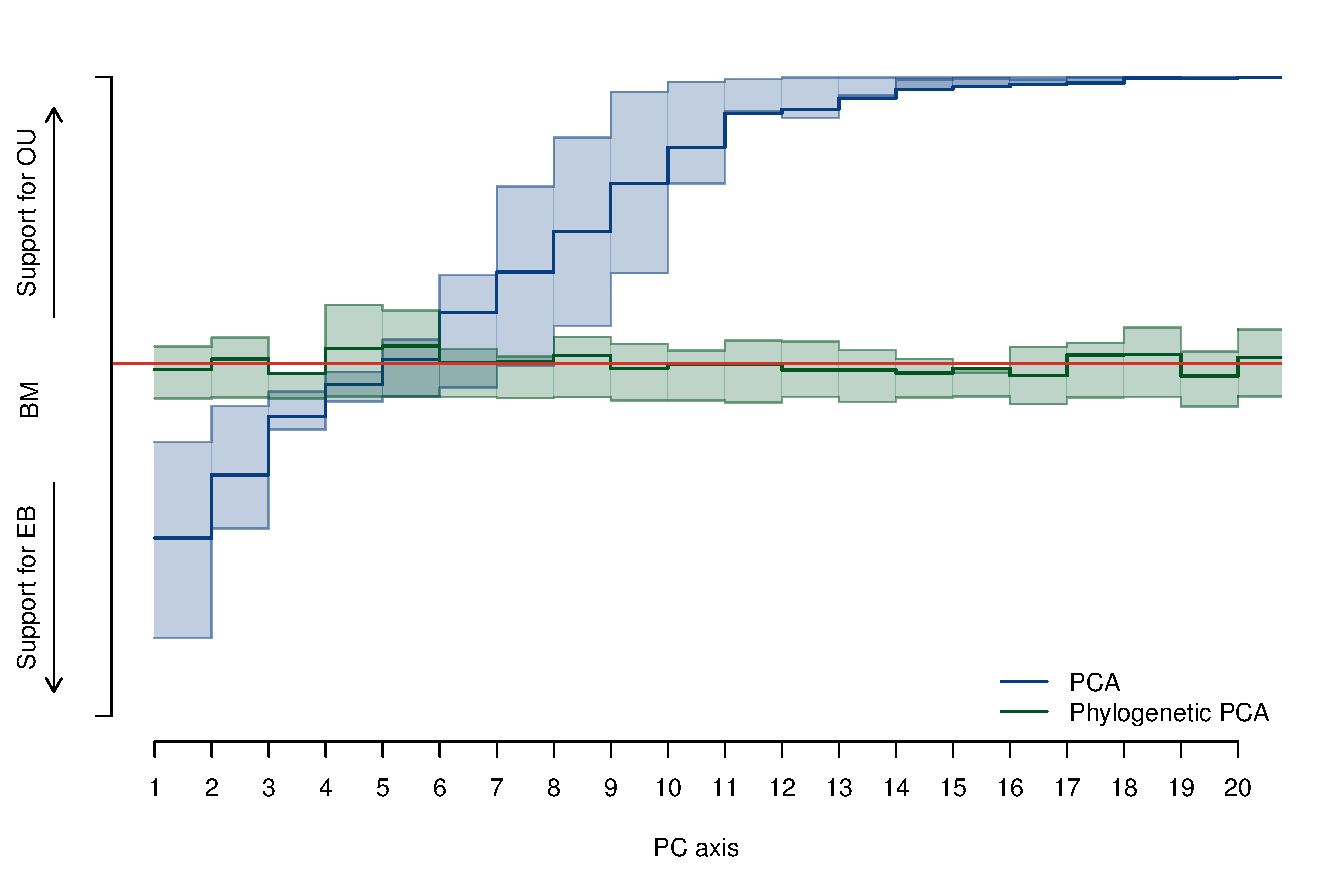
\includegraphics[scale=0.65]{./fig/mv-bm-aic.pdf}
\caption{Distribution of support for BM, OU and EB models when the generating model is a correlated multivariate BM model. Support for models were transformed into a linear scale by calculating an overall model support statistic: $AICw_{OU} - AICw_{EB}$. Thus high values support OU, low values support EB, and intermediate values near 0 indicate BM-like evolution. Models were fit to each replicated dataset for each of 20 different traits which were taken either from PC scores (blue line) or phylogenetic PC scores (green line). Shaded regions indicate the one standard deviation from the mean model-support statistic for  100 replicated datasets. The red  line indicates the average model support statistic averaged over all 20 original trait variables. Note that EB models have higher Akaike weights for the first few PCs of standard PCA, and that later PCs subsequently favor BM and finally, OU models. No such bias is found across traits for either the original data or pPCA.}
\label{corbm}
\end{figure}

\begin{figure}[p]
\centering
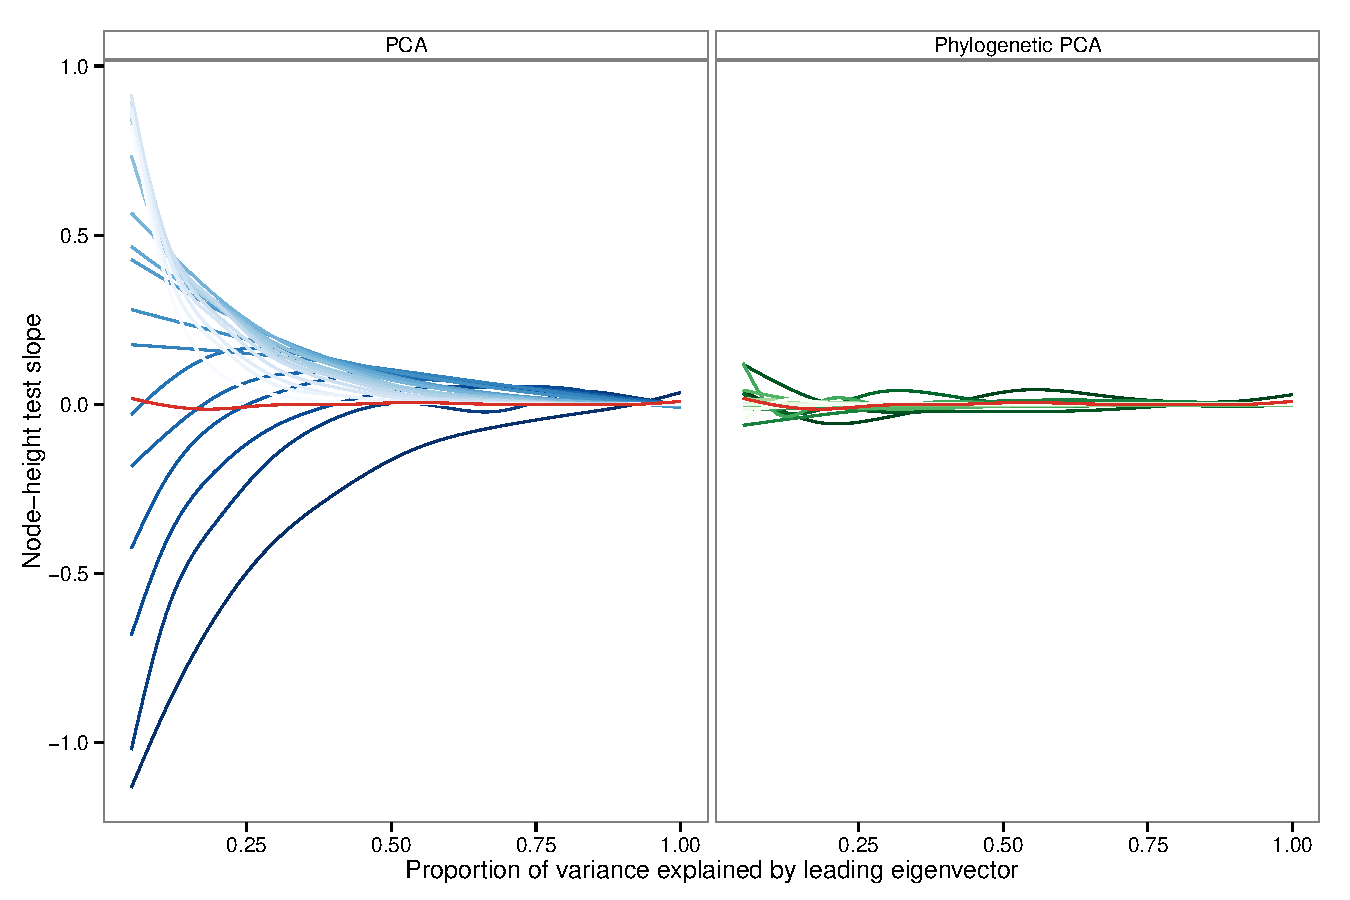
\includegraphics[scale=0.65]{./fig/onion.pdf}
\caption{Effect of trait correlations on the slope of the node height test for PC scores (left) and pPC scores (right) under a multivariate BM model of evolution. The red line is the aggregated data for all 20 traits on the original (untransformed) scale. When the leading eigenvector explains very little variation in the data and the effective dimensionality is high, the slope of node height test increases from negative to positive across PC axes. This indicates that under standard PCA, PC1 has higher contrasts near the root of the tree, while later PCs have higher contrasts near the tips (resulting in the pattern of model support observed in Figure ~\ref{corbm}). As the amount of variance explained by the principal eigenvector increases, the slope of the node height test approaches 0. No such effect is found for phylogenetic PCA.}
\label{rank}
\end{figure}

%\caption{Akaike weights (AICw) and parameter estimates for data simulated under an OU model, but subsequently fit %to pPCA scores assuming multivariate BM. Akaike weights across traits (either original data, or pPCs) show a %regular pattern of increasing support for BM and EB  moving down pPCA axes (top panel). Furthermore, while $\alpha$ %and other parameters are well--estimated for the original traits, pPCA produces a regular pattern of decreasing %$\alpha$ values across pPC scores (bottom panel). Note that the first few pPC axes have strong support for an OU %model, and substantially higher estimates of $\alpha$ relative to the value used to generate the data (solid blue %line, $\alpha = 2$).}
\begin{figure}[p]
\centering
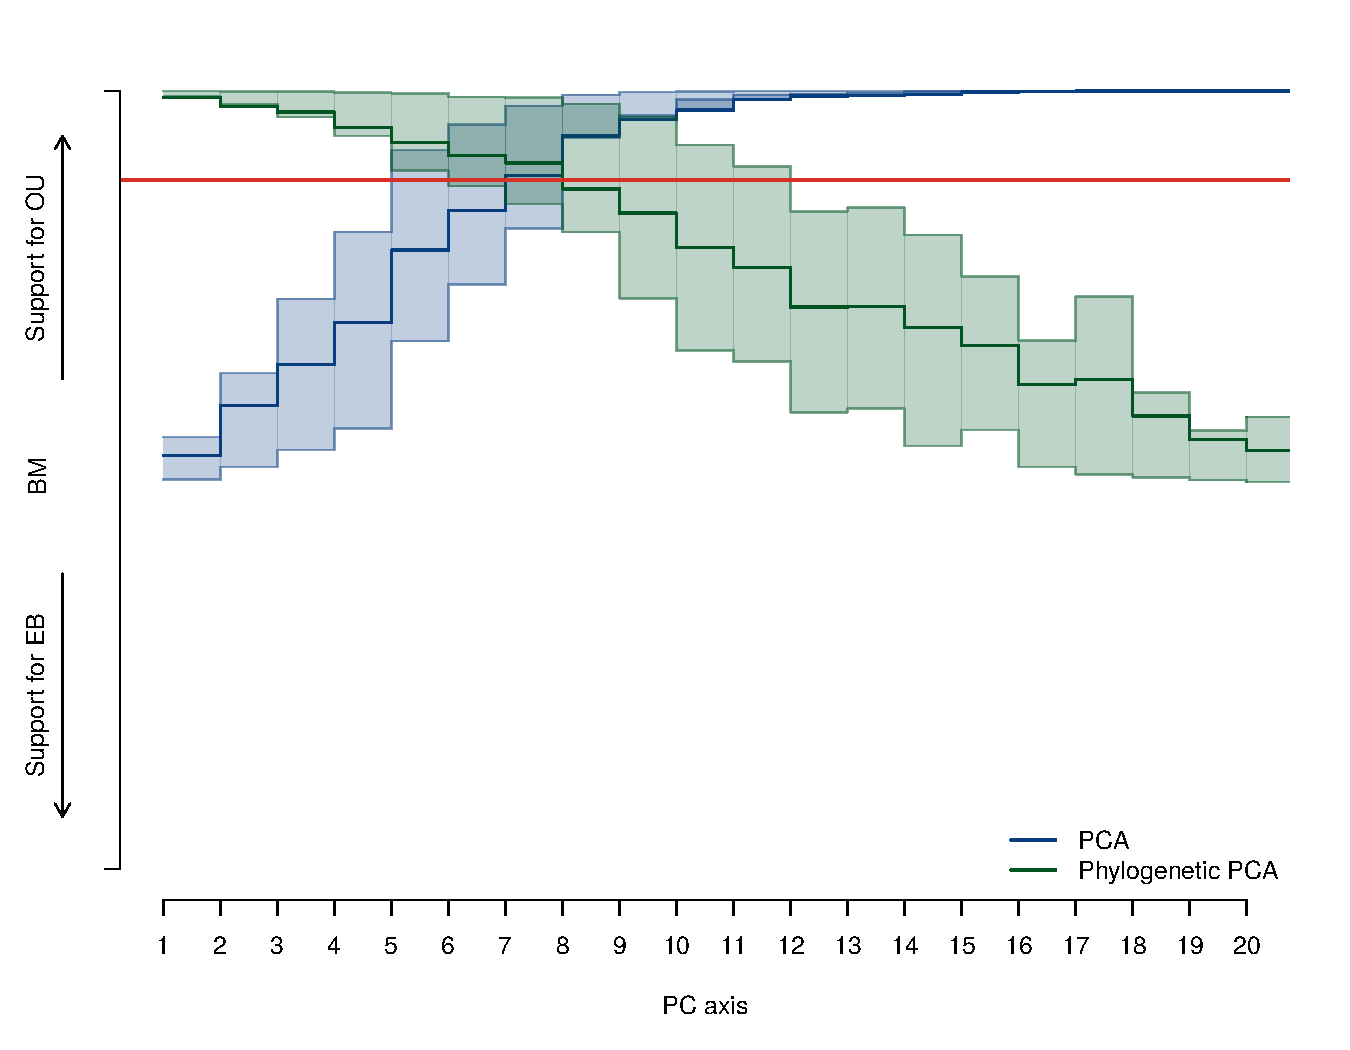
\includegraphics[scale=0.65]{./fig/uncor-ou-aic.pdf}
\caption{Distribution of support for BM, OU and EB models when the generating model is a uncorrelated multivariate OU model. Support for models were transformed into a linear scale by calculating an overall model support statistic: $AICw_{OU} - AICw_{EB}$. Thus high values support OU, low values support EB, and intermediate values near 0 indicate BM-like evolution. Models were fit to each replicated dataset for each of 20 different traits which were taken either from PC scores (blue line) or phylogenetic PC scores (green line). Shaded regions indicate the 25$^{th}$ and 75$^{th}$ quantiles of the mode--support statistic for  100 replicated datasets. The red  line indicates the average model support statistic averaged over all 20 original trait variables. Note that EB models have higher Akaike weights for the first few PCs of standard PCA, and that later PCs subsequently favor BM and finally, OU models. No such bias is found across traits for either the original data or pPCA.}
\label{oufit}
\end{figure}

\begin{figure}[p]
\centering
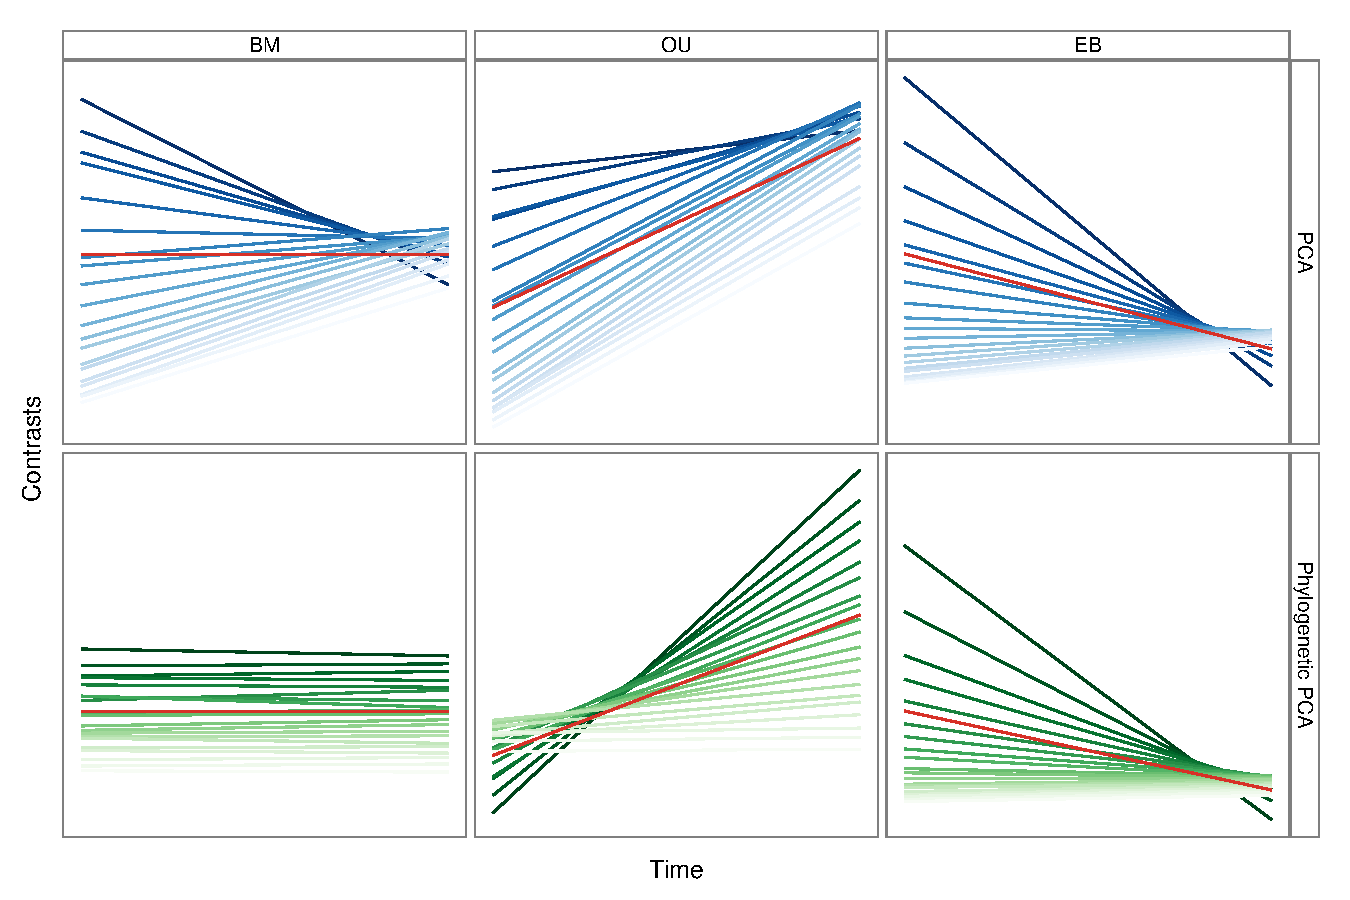
\includegraphics[scale=0.65]{./fig/nh-2panel.pdf}
\caption{Relationship between the average phylogenetic independent contrasts and the height of the node across 100 datasets simulated under either a BM (left), OU (middle) or EB (right) model of evolution. Contrasts were calculated for each of the 20 traits corresponding to either PC scores (top row) or pPPC scores (bottom row). Each line represents a best--fit linear model to the aggregated data across all 100 replicate simulations. Red lines are aggregated over all 20 traits on the original data. The plots are oriented so that the left side of each panel corresponds to the root of the phylogeny, with time increasing tipward to the right. PCA results in a predictable pattern of increasing slope in the contrasts across PCs. By contrast, pPCA only has systematic distortions across pPC axes when the underlying model is not multivariate BM. When this occurs, the first few pPC axes tend to have more extreme slopes than the original data (but in the correct direction).}
\label{nhplot}
\end{figure}

\begin{figure}[p]
\centering
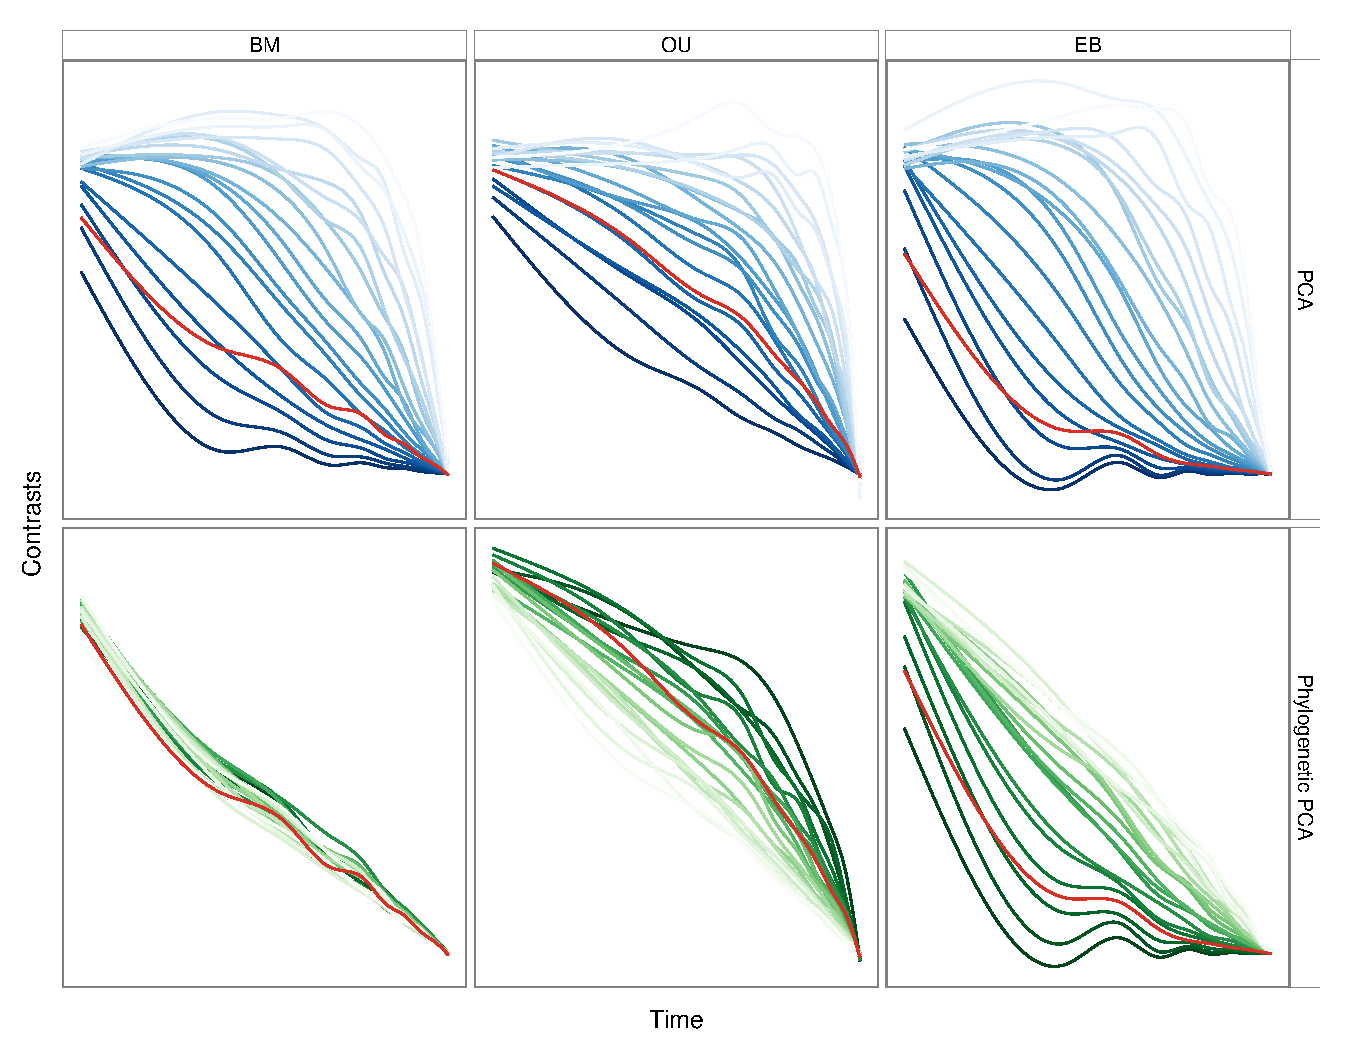
\includegraphics[scale=0.65]{./fig/dtt-2panel.pdf}
\caption{Disparity through time plots averaged across the 100 simulated datasets. The datasets were simulated under BM (left), OU (middle) or EB (right). The analyses were then performed on PC scores (top row) and pPPC scores (bottom row). The average disparity through time of all 20 original trait variables is indicated by the red line. We fit a loess curve through the relative disparities for each trait/transformation/model combination. The plots are oriented so that the left side of each panel corresponds to the root of the phylogeny, with time increasing tipward to the right. As in Fig. \ref{nhplot}, the first few axes from the PCA show a strong pattern of high disparity early in the clades' histories with the higher components showing seemingly higher disparity towards the present. PPCA corrects the distortion if the generating model is multivariate BM. However, if the generating model was not BM, the first few pPC axes tend to show an exaggerated pattern of disparity relative to the original traits.}
\label{dttplot}
\end{figure}

\renewcommand\thefigure{S\arabic{figure}}
\renewcommand\thetable{S \arabic{table}}
\setcounter{figure}{0}    
\setcounter{table}{0}

\begin{figure}[p]
\centering
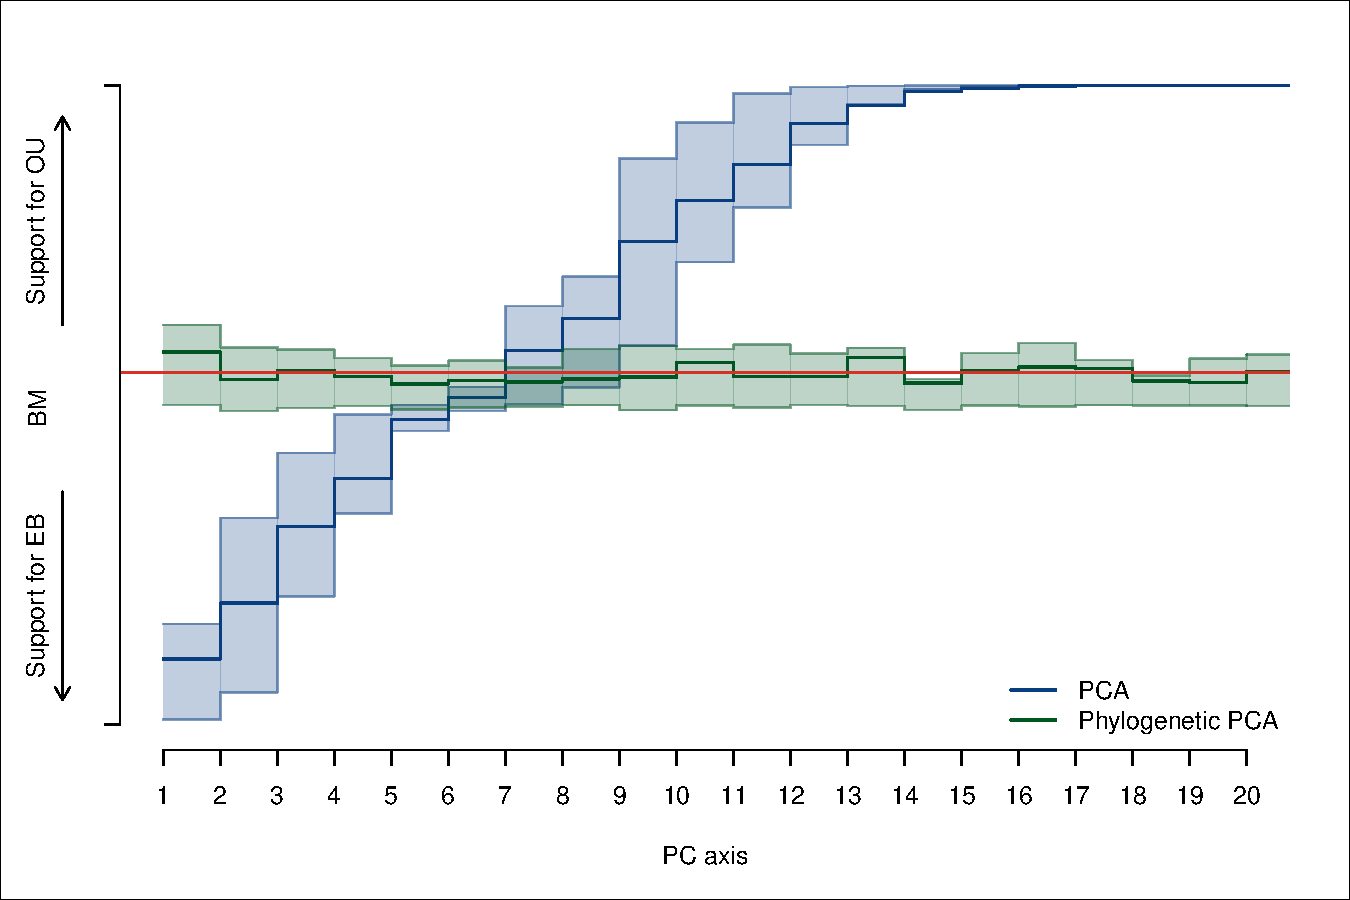
\includegraphics[scale=0.65]{./fig/uncor-bm-aic.pdf}
\caption{Distribution of support for BM, OU and EB models when the generating model is an uncorrelated multivariate BM model. Support for models were transformed into a linear scale by calculating an overall model support statistic: $AICw_{OU} - AICw_{EB}$. Thus high values support OU, low values support EB, and intermediate values near 0 indicate BM-like evolution. Models were fit to each replicated dataset for each of 20 different traits which were taken either from PC scores (blue line) or phylogenetic PC scores (green line). Shaded regions indicate the  25$^{th}$ and 75$^{th}$ quantiles of the mode--support statistic for  100 replicated datasets. The red  line indicates the average model support statistic averaged over all 20 original trait variables. Note that EB models have higher Akaike weights for the first few PCs of standard PCA, and that later PCs subsequently favor BM and finally, OU models. No such bias is found across traits for either the original data or pPCA.}
\label{aicwbm}
\end{figure}

\begin{figure}[p]
\centering
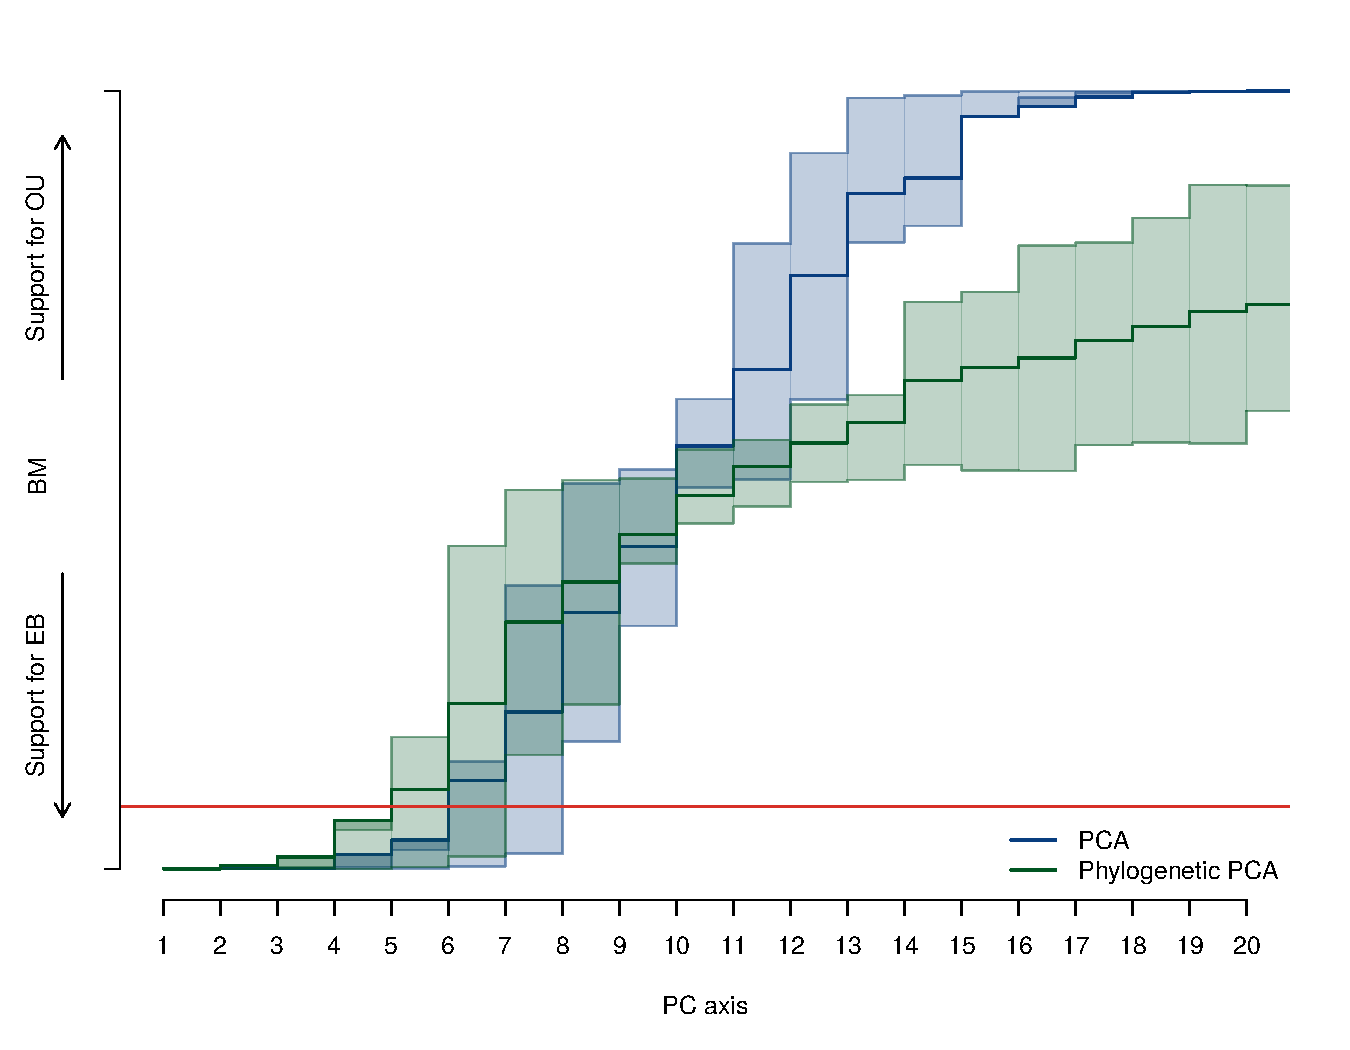
\includegraphics[scale=0.65]{./fig/uncor-eb-aic.pdf}
\caption{Distribution of support for BM, OU and EB models when the generating model is a uncorrelated multivariate EB model. Support for models were transformed into a linear scale by calculating an overall model support statistic: $AICw_{OU} - AICw_{EB}$. Thus high values support OU, low values support EB, and intermediate values near 0 indicate BM-like evolution. Models were fit to each replicated dataset for each of 20 different traits which were taken either from PC scores (blue line) or phylogenetic PC scores (green line). Shaded regions indicate the 25$^{th}$ and 75$^{th}$ quantiles of the model--support statistic for 100 replicated datasets. The red  line indicates the average model support statistic averaged over all 20 original trait variables. Note that EB models have higher Akaike weights for the first few PCs of standard PCA, and that later PCs subsequently favor BM and finally, OU models. No such bias is found across traits for either the original data or pPCA.}
\label{aicweb}
\end{figure}

\begin{figure}[p]
\centering
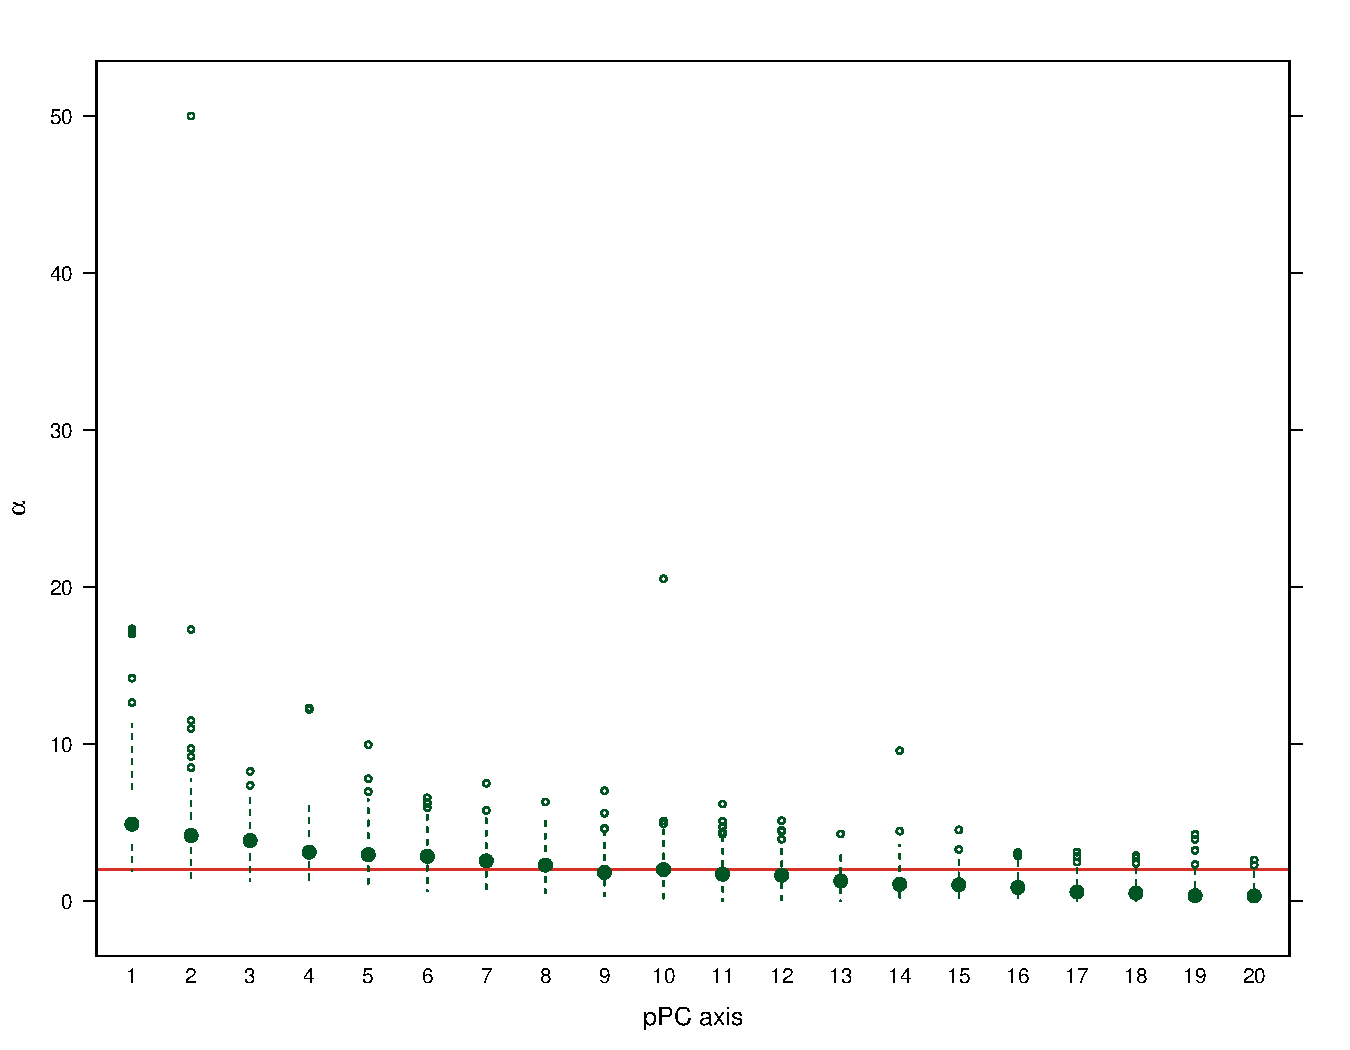
\includegraphics[scale=0.65]{fig/alpha-est.pdf}
\caption{Estimated values of the $\alpha$ parameter from phylogenetic PCA when data is simulated under an uncorrelated multivariate OU model. The simulating value $\alpha=$2 is depicted with the red line. The estimate of $\alpha$ is inflated in the first few pPC axes consistent with an exaggerated support for the OU model. In the last pPC axes, $\alpha$ is estimated to be very close to 0, such that the OU model is statistically indistinguishable from a BM model. These results mirror those depicted in Figure \ref{oufit}.}
\label{alpha}
\end{figure}

\end{document}
